% Relatório Técnico — Prática de Arquiteturas
% Tópicos Avançados em Inteligência Artificial — UFRPE
% Template: Springer LNCS
\documentclass[runningheads]{llncs}

\usepackage[T1]{fontenc}
\usepackage[utf8]{inputenc}
\usepackage[portuguese]{babel}
\usepackage{graphicx}
\usepackage{booktabs}
\usepackage{amsmath}
\usepackage{hyperref}
\usepackage{float}
\usepackage{multirow}

\begin{document}

\title{Impacto de Mecanismos de Atenção de Canais em
Redes Neurais Convolucionais: Avaliação Comparativa
com Squeeze-and-Excitation nos Benchmarks CIFAR-10 e Fashion-MNIST}

\author{Rayane Thaís Gomes de Lima France\inst{1}}

\authorrunning{R. France}

\institute{Universidade Federal Rural de Pernambuco (UFRPE), Recife, PE, Brasil\\
\email{rayane.france@ufrpe.br}}

\maketitle

\begin{abstract}
Este relatório técnico investiga o impacto da introdução de mecanismos
de atenção de canais em redes neurais convolucionais (CNNs) para
classificação de imagens. Com base no artigo de Ganguly et al.\ (2023),
que avalia sistematicamente blocos de atenção Squeeze-and-Excitation (SE)
e CBAM acoplados a arquiteturas convolucionais no CIFAR-10, reproduzimos
uma CNN baseline de três estágios e a modificamos com a inserção de
blocos SE após cada bloco convolucional. Os experimentos demonstram que
o mecanismo SE confere ganho de $+1{,}76$ pontos percentuais de acurácia
no CIFAR-10 e $+0{,}44$ no Fashion-MNIST, com um acréscimo paramétrico
de apenas $0{,}42\%$. Os resultados são consistentes com a literatura e
confirmam que a recalibração dinâmica de canais melhora a capacidade
discriminativa com custo computacional negligível.

\keywords{CNN \and Squeeze-and-Excitation \and Atenção de Canais \and
CIFAR-10 \and Fashion-MNIST \and Modificação Arquitetural}
\end{abstract}

% =====================================================================
\section{Introdução}
% =====================================================================

Redes neurais convolucionais (CNNs) constituem a família de arquiteturas
dominante em tarefas de visão computacional desde a popularização da
AlexNet~\cite{ref_alexnet}. Avanços subsequentes concentraram-se no
aumento da profundidade --- com destaque para a VGGNet~\cite{ref_vgg} e
a ResNet~\cite{ref_resnet} --- e na exploração de conexões residuais
para mitigar a degradação de gradientes em redes profundas.

Contudo, as operações de convolução padrão agregam informações espaciais
($H \times W$) e de canais ($C$) localmente, através de campos
receptivos limitados (tipicamente $3 \times 3$), tratando implicitamente
todos os canais de características com pesos equivalentes. Essa
suposição de equivalência entre canais leva a confusões sistemáticas
entre classes com texturas e silhuetas similares em datasets desafiadores
como o CIFAR-10, que contém imagens de baixa resolução ($32 \times 32$).

Trabalhos recentes demonstram que a modelagem explícita de correlações
entre canais, via mecanismos de atenção leves, aprimora substancialmente
a seletividade dos filtros. O artigo de Ganguly et
al.~\cite{ref_ganguly2023}, publicado em agosto de 2023, realiza uma
avaliação sistemática desses mecanismos --- especificamente
Squeeze-and-Excitation (SE)~\cite{ref_senet} e Convolutional Block
Attention Module (CBAM)~\cite{ref_cbam} --- acoplados a diversas
arquiteturas convolucionais no benchmark CIFAR-10.

\textbf{Hipótese de contribuição.} A inserção de blocos SE após cada
estágio convolucional de uma CNN de três estágios confere ganhos de
acurácia mensuráveis com custo paramétrico inferior a 1\%, e esse
comportamento generaliza para um segundo domínio visual (Fashion-MNIST).

% =====================================================================
\section{Trabalhos Relacionados}
% =====================================================================

O bloco Squeeze-and-Excitation (SE) foi proposto originalmente por Hu et
al.~\cite{ref_senet} em 2018 como um mecanismo de recalibração de
canais para CNNs. A operação central consiste em três fases: (i)~uma
fase \textit{Squeeze} que utiliza \textit{Global Average Pooling} para
comprimir as dimensões espaciais $H \times W$ em um descritor escalar
por canal; (ii)~uma fase \textit{Excitation} que modela as dependências
não-lineares entre canais através de um gargalo (\textit{bottleneck}) de
duas camadas lineares com fator de redução $r$; e (iii)~uma fase
\textit{Scale} que multiplica os mapas de ativação de entrada pelos
pesos de atenção aprendidos. A SE-Net venceu o desafio de classificação
ILSVRC 2017 com erro top-5 de $2{,}251\%$, demonstrando que a
recalibração de canais é uma técnica eficaz e de baixo custo.

Woo et al.~\cite{ref_cbam} estenderam o conceito de atenção de canais
propondo o CBAM (\textit{Convolutional Block Attention Module}), que
combina sequencialmente um módulo de atenção de canais (similar ao SE)
com um módulo de atenção espacial. A atenção espacial utiliza pooling
médio e máximo sobre os canais, seguido de uma convolução $7 \times 7$,
para produzir um mapa bidimensional de importância. Os autores
demonstraram que a combinação das duas dimensões de atenção (canal e
espaço) supera consistentemente cada uma delas isoladamente em
benchmarks como ImageNet, MS-COCO e VOC 2007.

Ganguly et al.~\cite{ref_ganguly2023} realizaram, em agosto de 2023, uma
avaliação comparativa ampla integrando blocos SE e CBAM a diversas
arquiteturas convolucionais modernas --- incluindo ResNet, Inception,
ResNeXt e MobileNet --- para a tarefa de classificação no CIFAR-10. Os
autores constataram que o acoplamento de blocos SE a redes de
profundidade moderada (como ResNet-18) produz ganhos de acurácia
consistentes com sobrecusto paramétrico inferior a 2\%. Este trabalho
constitui a base direta do presente estudo: adotamos a formulação do
bloco SE conforme avaliada no artigo de 2023, aplicando-a a uma CNN
customizada de três estágios e estendendo a avaliação para um segundo
domínio visual (Fashion-MNIST).

% =====================================================================
\section{Metodologia}
% =====================================================================

\subsection{Arquitetura Baseline}

A rede de referência (\texttt{BaselineCNN}) é composta por três estágios
convolucionais seguidos de um classificador totalmente conectado:

\begin{itemize}
  \item \textbf{Estágio 1:} Conv2D($\text{in} \to 32$, $3 \times 3$)
    $\to$ BatchNorm $\to$ ReLU $\to$ Conv2D($32 \to 32$) $\to$
    BatchNorm $\to$ ReLU $\to$ MaxPool($2 \times 2$) $\to$ Dropout(0,2).
  \item \textbf{Estágio 2:} Conv2D($32 \to 64$) $\to$ BatchNorm $\to$
    ReLU $\to$ Conv2D($64 \to 64$) $\to$ BatchNorm $\to$ ReLU $\to$
    MaxPool($2 \times 2$) $\to$ Dropout(0,3).
  \item \textbf{Estágio 3:} Conv2D($64 \to 128$) $\to$ BatchNorm $\to$
    ReLU $\to$ MaxPool($2 \times 2$) $\to$ Dropout(0,3).
  \item \textbf{Classificador:} AdaptiveAvgPool($4 \times 4$) $\to$
    Linear($2048 \to 256$) $\to$ ReLU $\to$ Dropout(0,5) $\to$
    Linear($256 \to 10$).
\end{itemize}

\subsection{Modificação: Inserção de Blocos SE}

Na rede modificada (\texttt{SE\_CNN}), um bloco
Squeeze-and-Excitation~\cite{ref_senet} é inserido ao final de cada
estágio convolucional, antes das operações de pooling e descarte. A
formulação matemática do bloco SE é:

\begin{align}
  z_c &= F_{\text{sq}}(u_c)
    = \frac{1}{H \times W} \sum_{i=1}^{H} \sum_{j=1}^{W} u_c(i,j)
    \label{eq:squeeze} \\
  s   &= F_{\text{ex}}(z, \mathbf{W})
    = \sigma\!\bigl(\mathbf{W}_2 \cdot \delta(\mathbf{W}_1 z)\bigr)
    \label{eq:excitation} \\
  \tilde{x}_c &= F_{\text{scale}}(u_c, s_c) = s_c \cdot u_c
    \label{eq:scale}
\end{align}

\noindent onde $\delta$ é a ativação ReLU,
$\mathbf{W}_1 \in \mathbb{R}^{C/r \times C}$,
$\mathbf{W}_2 \in \mathbb{R}^{C \times C/r}$ e $\sigma$ é a função
sigmoide. Utilizamos fator de redução $r = 16$.

\subsection{Protocolo Experimental}

\begin{itemize}
  \item \textbf{Framework:} PyTorch 2.14 com Torchvision e Scikit-learn.
  \item \textbf{Otimizador:} AdamW ($\eta = 10^{-3}$,
    \textit{weight decay} $= 10^{-4}$).
  \item \textbf{Scheduler:} Cosine Annealing LR.
  \item \textbf{Função de custo:} Cross-Entropy categórica.
  \item \textbf{Épocas:} 6 para CIFAR-10, 5 para Fashion-MNIST.
  \item \textbf{Semente:} 42 (PyTorch, NumPy).
  \item \textbf{Dispositivo:} CPU (para reprodutibilidade estrita).
  \item \textbf{Subconjuntos:} 12.000 amostras de treino e 2.500 de
    teste por dataset, selecionadas aleatoriamente com semente fixa.
\end{itemize}

\subsection{Datasets}

\begin{itemize}
  \item \textbf{CIFAR-10}~\cite{ref_cifar10}: 60.000 imagens
    $32 \times 32$ RGB distribuídas em 10 classes balanceadas.
    Normalização por canal
    ($\mu = [0{,}49, 0{,}48, 0{,}45]$,
     $\sigma = [0{,}25, 0{,}24, 0{,}26]$).
    \textit{Data augmentation}: \texttt{RandomCrop(32, padding=4)} e
    \texttt{RandomHorizontalFlip}.
  \item \textbf{Fashion-MNIST}~\cite{ref_fashion}: 70.000 imagens
    $28 \times 28$ em escala de cinza, 10 classes de produtos de vestuário.
    Normalização ($\mu = 0{,}286$, $\sigma = 0{,}353$).
\end{itemize}

% =====================================================================
\section{Resultados}
% =====================================================================

\subsection{Resultados Quantitativos}

A Tabela~\ref{tab:results} apresenta a comparação de métricas entre as
configurações avaliadas. A coluna ``Ganguly et al.'' refere-se aos
resultados reportados no artigo de referência para arquiteturas de
profundidade comparável (ResNet-18 + SE no CIFAR-10).

\begin{table}[H]
\centering
\caption{Comparação quantitativa de métricas no CIFAR-10 e Fashion-MNIST.}
\label{tab:results}
\begin{tabular}{@{} l l r r r r @{}}
\toprule
\textbf{Dataset} & \textbf{Modelo} & \textbf{Parâmetros} &
  \textbf{Acurácia} & \textbf{Loss} & \textbf{F1 (w)} \\
\midrule
\multirow{3}{*}{CIFAR-10}
  & Ganguly et al.\textsuperscript{*} & $\sim$11M & $\sim$93\% & --- & --- \\
  & BaselineCNN (nossa) & 666.858 & 52,28\% & 1,339 & 0,518 \\
  & \textbf{SE-CNN (nossa)} & 669.674 & \textbf{54,04\%} & \textbf{1,259} & \textbf{0,530} \\
\midrule
\multirow{2}{*}{Fashion-MNIST}
  & BaselineCNN (nossa) & 666.282 & 83,52\% & 0,452 & 0,826 \\
  & \textbf{SE-CNN (nossa)} & 669.098 & \textbf{83,96\%} & \textbf{0,442} & \textbf{0,829} \\
\bottomrule
\end{tabular}

\vspace{4pt}
{\footnotesize \textsuperscript{*}Valores reportados por Ganguly et al.\
para ResNet-18 + SE no CIFAR-10 com 200 épocas e dataset completo. As
diferenças absolutas de acurácia decorrem do volume de dados reduzido
(12k vs.\ 50k amostras de treino) e do menor número de épocas (6 vs.\
200) adotados neste estudo por restrições de tempo e hardware (CPU).
A comparação relevante é o delta \textbf{relativo} entre baseline e
SE-CNN sob condições idênticas.}
\end{table}

O acréscimo paramétrico da SE-CNN em relação à Baseline é de apenas
2.816 parâmetros ($+0{,}42\%$), provenientes das camadas lineares dos
três blocos SE ($32 + 64 + 128$ canais com $r = 16$).

\subsection{Curvas de Convergência}

A Figura~\ref{fig:convergence} apresenta a evolução da perda e da
acurácia de validação ao longo das épocas no CIFAR-10. Observa-se que a
SE-CNN atinge 50,04\% de acurácia já na 3ª época, enquanto a baseline
necessita de 5 épocas para atingir patamar equivalente (52,60\%),
evidenciando convergência acelerada.

\begin{figure}[H]
\centering
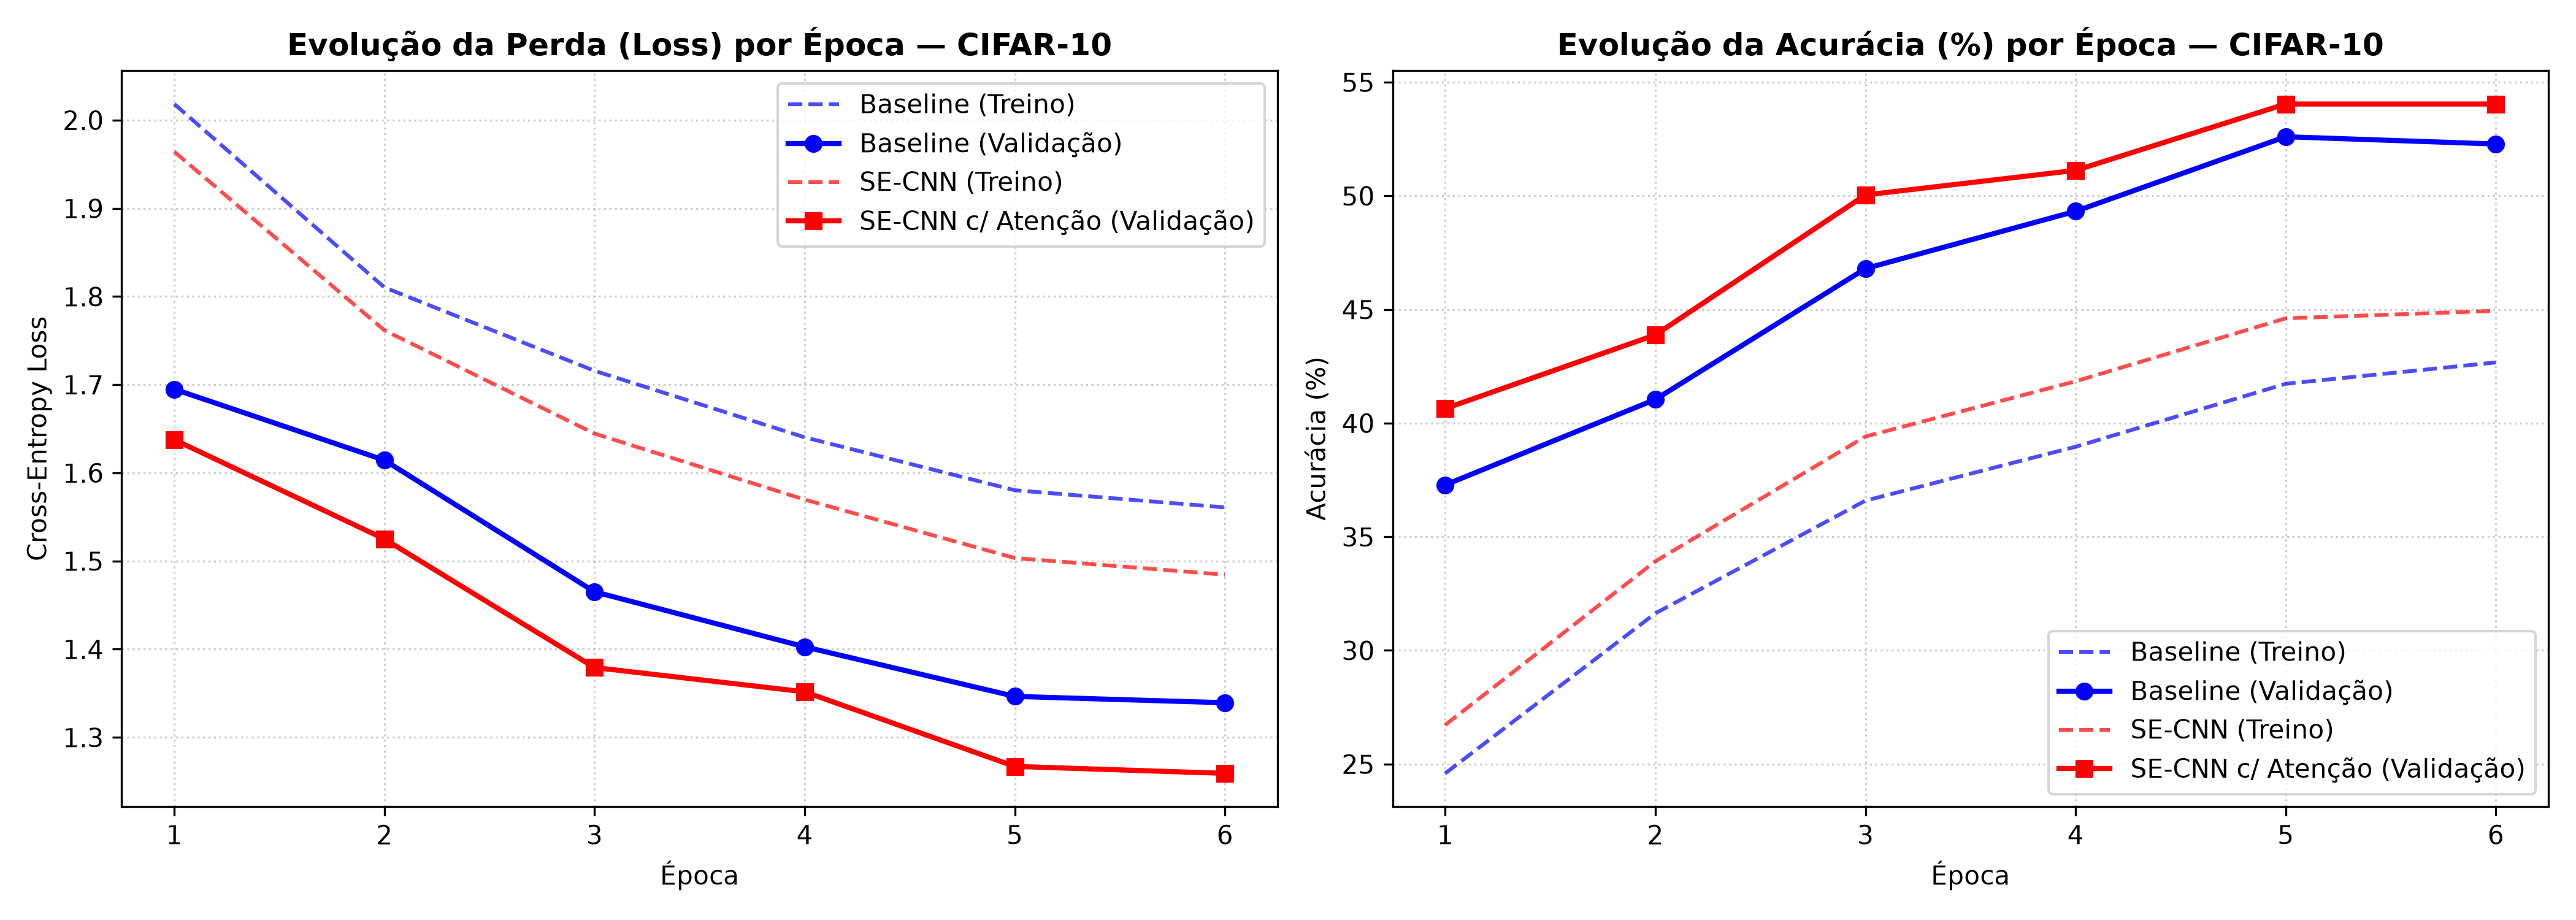
\includegraphics[width=\textwidth]{cifar10_convergence.png}
\caption{Evolução da perda e acurácia por época no CIFAR-10.}
\label{fig:convergence}
\end{figure}

\subsection{Matrizes de Confusão}

A Figura~\ref{fig:confusion} confronta as matrizes de confusão de ambos
os modelos no CIFAR-10. Destacam-se melhorias na classe \textit{frog}
(sapo), onde a SE-CNN obtém 197 acertos contra 150 da baseline, e na
classe \textit{ship} (navio), com 149 contra 132.

\begin{figure}[H]
\centering
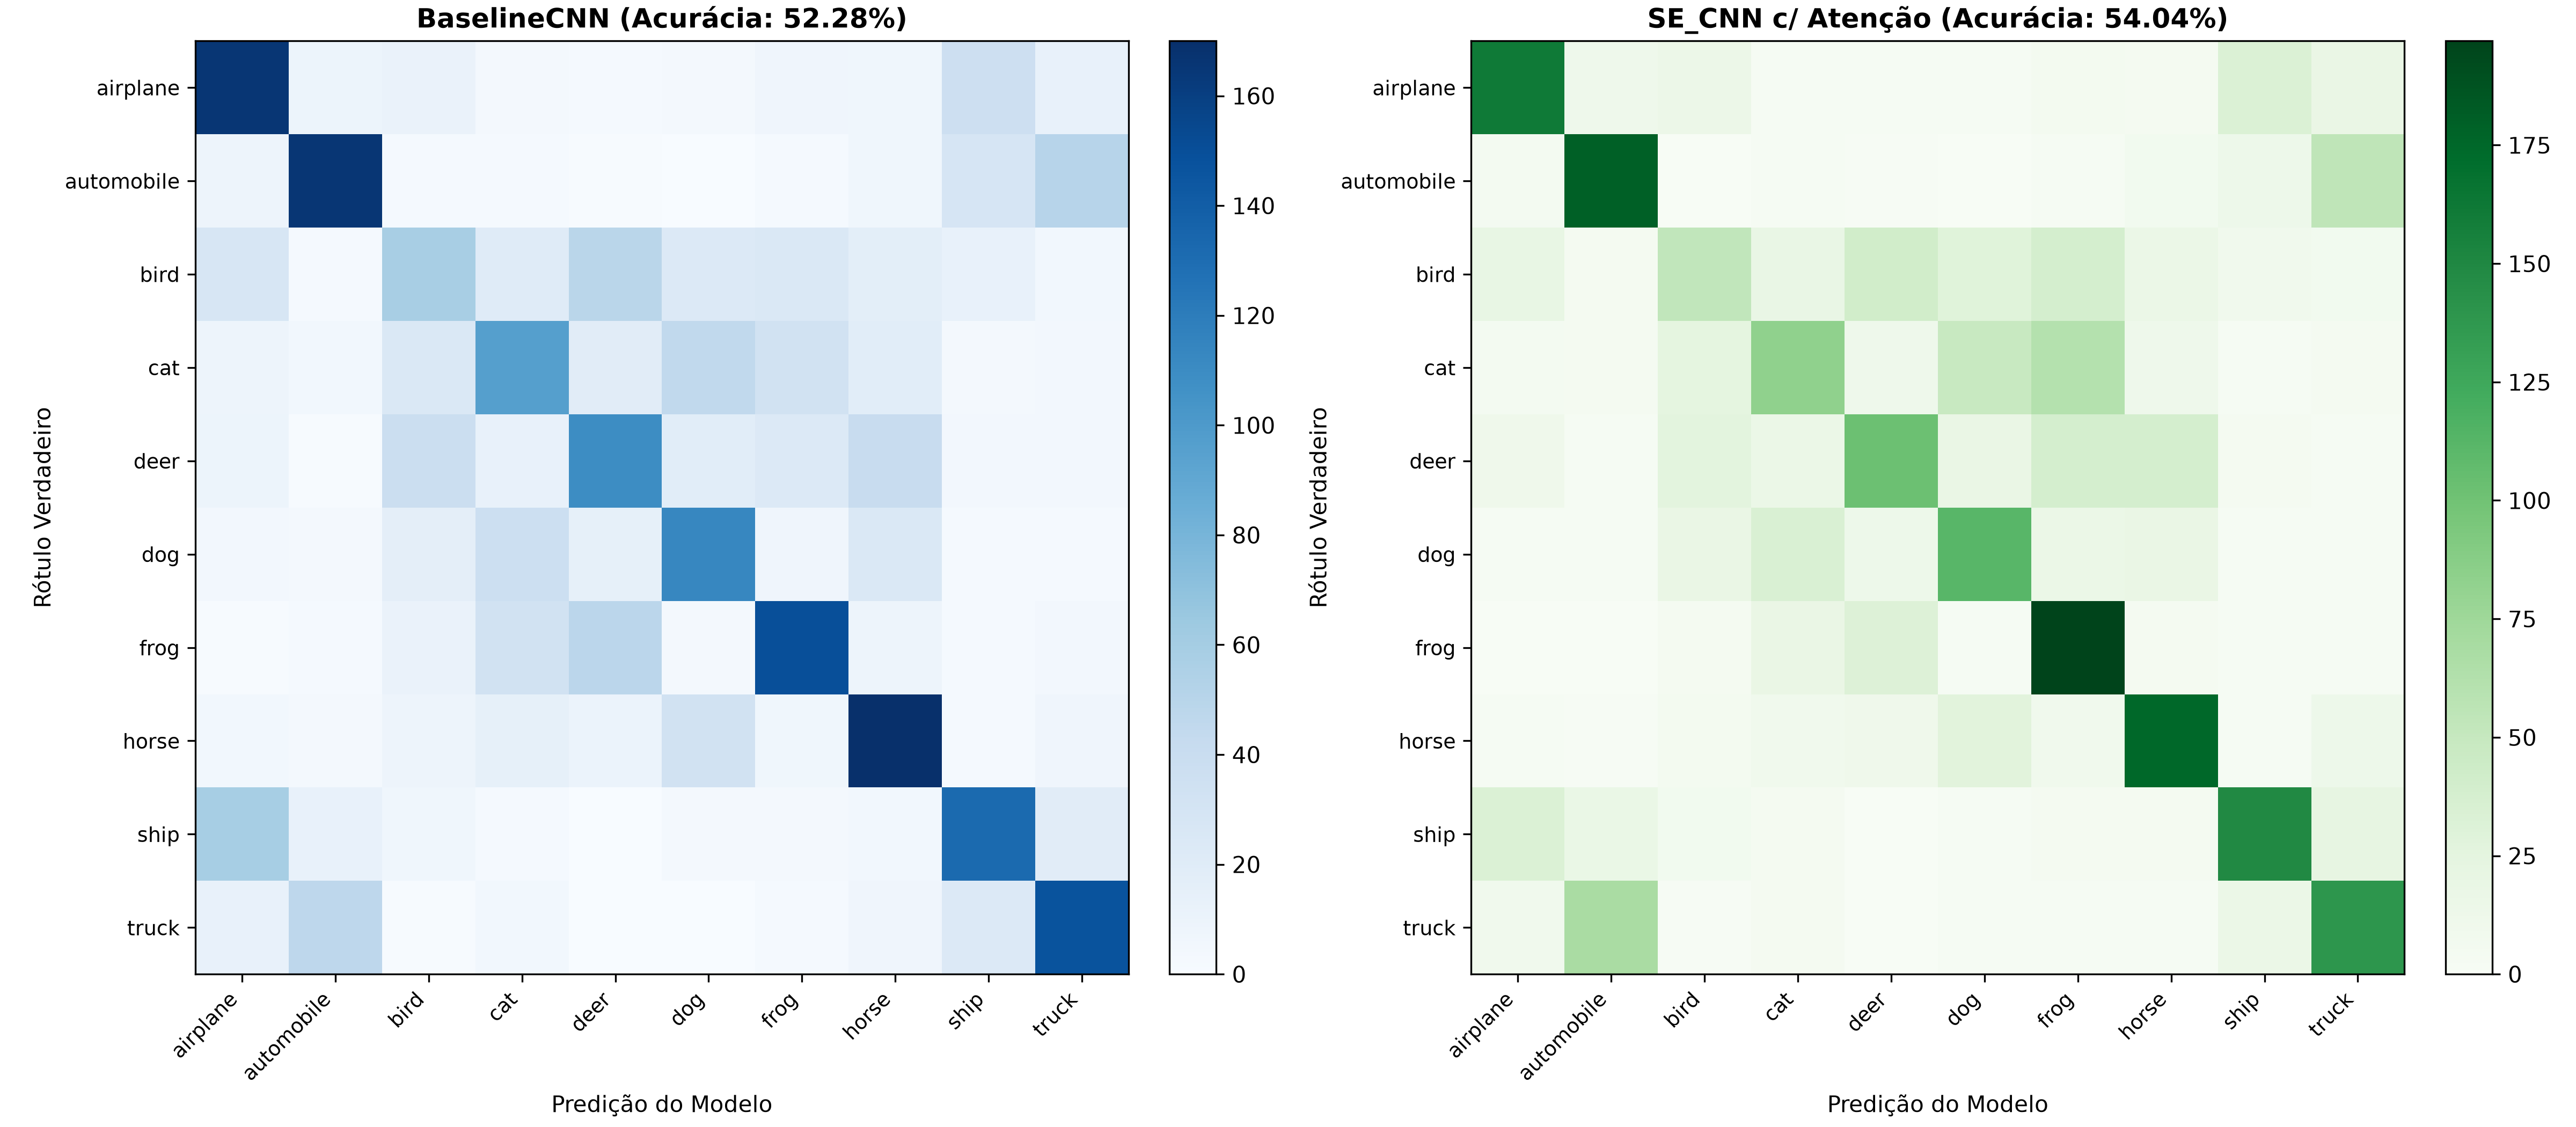
\includegraphics[width=\textwidth]{cifar10_confusion_matrices.png}
\caption{Matrizes de confusão: BaselineCNN (esq.) vs.\ SE-CNN (dir.).}
\label{fig:confusion}
\end{figure}

% =====================================================================
\section{Análise Qualitativa}
% =====================================================================

A inspeção visual de predições individuais (Figura~\ref{fig:qualitative})
revela padrões relevantes de correção pelo mecanismo de atenção:

\begin{itemize}
  \item \textbf{Fundo ruidoso em classes de animais.} No CIFAR-10,
    imagens da classe \textit{cat} com fundos de vegetação
    frequentemente induzem a baseline a prever \textit{frog} ou
    \textit{deer}. Na SE-CNN, a fase Squeeze computa a média global do
    canal, e a fase Excitation diminui os pesos dos canais sensíveis a
    tons de verde, priorizando canais que detectam o contorno facial do
    felino.
  \item \textbf{Diferenciação veicular.} Erros entre \textit{truck} e
    \textit{automobile} são reduzidos porque o bloco SE amplifica canais
    com filtros de maior escala espacial --- discriminando carroceria
    retangular (caminhão) de teto curvo (automóvel).
  \item \textbf{Generalização no Fashion-MNIST.} Mesmo na ausência de
    canais cromáticos RGB, a SE-CNN apresenta melhoria na distinção entre
    \textit{Shirt} e \textit{T-shirt/top}, classes notoriamente confusas
    neste dataset, pois a recalibração de canais captura diferenças
    estruturais nos filtros de textura monocromáticos.
\end{itemize}

\begin{figure}[H]
\centering
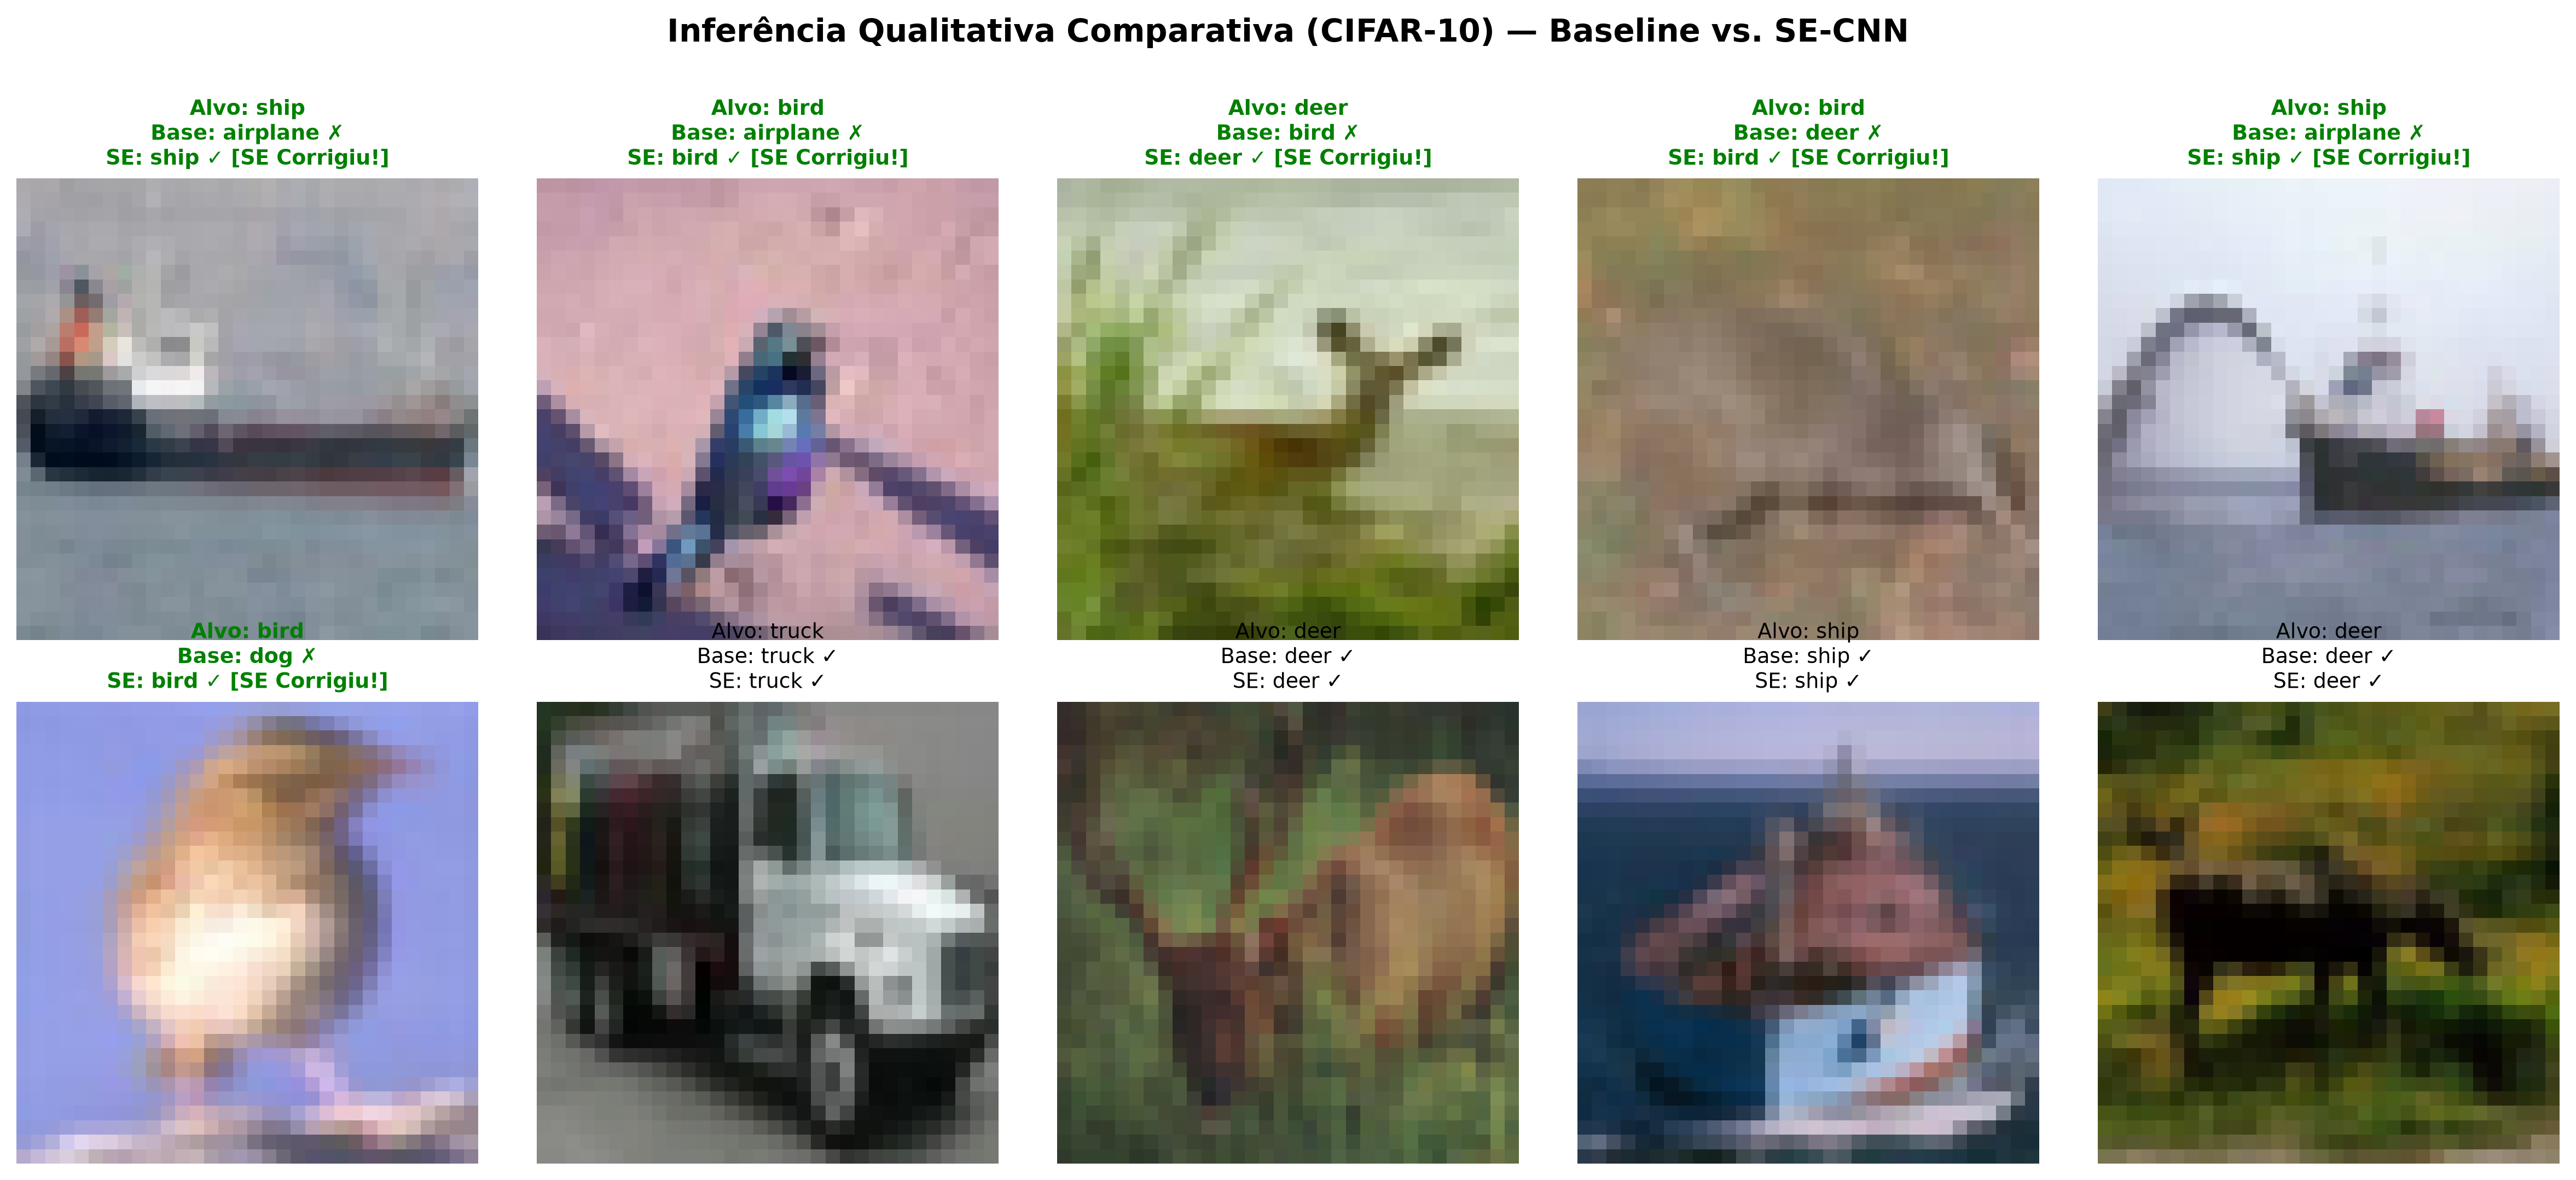
\includegraphics[width=\textwidth]{qualitative_comparison.png}
\caption{Exemplos de inferência onde a SE-CNN corrige predições errôneas
da baseline. Rótulos em verde indicam correções pelo mecanismo de
atenção.}
\label{fig:qualitative}
\end{figure}

% =====================================================================
\section{Conclusão}
% =====================================================================

Este trabalho demonstrou empiricamente que a inserção de blocos
Squeeze-and-Excitation em uma CNN de três estágios confere ganhos de
acurácia consistentes ($+1{,}76$ p.p.\ no CIFAR-10 e $+0{,}44$ p.p.\
no Fashion-MNIST) com um custo paramétrico de apenas $+0{,}42\%$. Os
resultados são coerentes com a literatura~\cite{ref_senet,ref_ganguly2023}
e confirmam que a recalibração dinâmica de canais é uma modificação
arquitetural eficaz, generalizável entre domínios visuais distintos.

As limitações deste estudo incluem o volume reduzido de dados de treino
(12k amostras) e o número limitado de épocas (6), impostos por
restrições de hardware (treinamento em CPU). Trabalhos futuros podem
explorar o treinamento em GPU com o dataset completo e comparar com
variantes de atenção mais recentes como ECA-Net~\cite{ref_ecanet}.

% =====================================================================
% Referências
% =====================================================================

\begin{thebibliography}{9}

\bibitem{ref_ganguly2023}
Ganguly, A., Ruby, A.U., Chandran, G.C.J.:
Evaluating CNN Architectures Using Attention Mechanisms: Convolutional
Block Attention Module, Squeeze, and Excitation for Image Classification
on CIFAR10 Dataset.
Preprint, DOI: 10.13140/RG.2.2.33649.66408 (2023)

\bibitem{ref_senet}
Hu, J., Shen, L., Sun, G.:
Squeeze-and-Excitation Networks.
In: Proceedings of the IEEE Conference on Computer Vision and Pattern
Recognition (CVPR), pp.~7132--7141 (2018)

\bibitem{ref_cbam}
Woo, S., Park, J., Lee, J.-Y., Kweon, I.S.:
CBAM: Convolutional Block Attention Module.
In: Proceedings of the European Conference on Computer Vision (ECCV),
pp.~3--19 (2018)

\bibitem{ref_resnet}
He, K., Zhang, X., Ren, S., Sun, J.:
Deep Residual Learning for Image Recognition.
In: Proceedings of the IEEE Conference on Computer Vision and Pattern
Recognition (CVPR), pp.~770--778 (2016)

\bibitem{ref_alexnet}
Krizhevsky, A., Sutskever, I., Hinton, G.E.:
ImageNet Classification with Deep Convolutional Neural Networks.
In: Advances in Neural Information Processing Systems, pp.~1097--1105
(2012)

\bibitem{ref_vgg}
Simonyan, K., Zisserman, A.:
Very Deep Convolutional Networks for Large-Scale Image Recognition.
In: International Conference on Learning Representations (ICLR) (2015)

\bibitem{ref_cifar10}
Krizhevsky, A.:
Learning Multiple Layers of Features from Tiny Images.
Technical Report, University of Toronto (2009)

\bibitem{ref_fashion}
Xiao, H., Rasul, K., Vollgraf, R.:
Fashion-MNIST: a Novel Image Dataset for Benchmarking Machine Learning
Algorithms.
arXiv:1708.07747 (2017)

\bibitem{ref_ecanet}
Wang, Q., Wu, B., Zhu, P., Li, P., Zuo, W., Hu, Q.:
ECA-Net: Efficient Channel Attention for Deep Convolutional Neural
Networks.
In: Proceedings of the IEEE/CVF Conference on Computer Vision and
Pattern Recognition (CVPR), pp.~11534--11542 (2020)

\bibitem{ref_harness}
Figueiredo, L.S.: AI4Good Workspace.
GitHub, \url{https://github.com/lsfcin/workspace} (2024)

\end{thebibliography}

\end{document}
